\chapter{Arquitectura y Diseño}


\section{Introducción}

Para poder ejecutar el agente, se desarrollaron un conjunto de aplicaciones que permiten la ejecución del algoritmo presentado en el capitulo anterior en un entorno simulado, que representara nuestro mercado financiero.
El código puede verse y descargarse desde \href{https://github.com/jcaramello/deepQ-stock}{\textcolor{blue}{github}}, en el también podrá encontrarse las instrucciones para su ejecución. El sistema implementado que acompaña a este documento, esta compuesto por dos soluciones principales, una aplicación cliente, desarrollada en Typescript y Angular 4, y una aplicación de backend, 
encargada de emular el mercado financiero y ejecutar los agentes en el.

\begin{figure}[h!]
	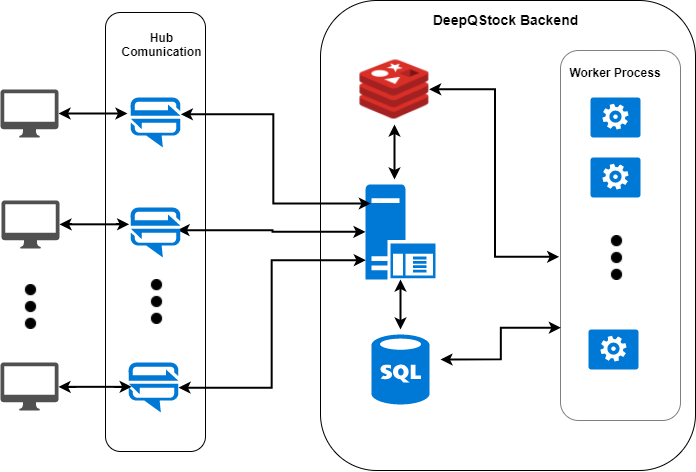
\includegraphics[scale=0.5]{imagenes/deepQStockArchitectureOverview.png}
	\caption{Arquitectura del sistema}
	\label{fig:cap4:1}
\end{figure}

\subsection{Aplicación cliente}
Esta aplicación permitirá crear agentes y sus entornos de simulación, permitiendo definir diferentes parámetros de configuración(Figura \ref{fig:cap4:2}), tanto del algoritmo de Q-learning como del entorno de simulación.\\ 

\begin{figure*}[h!]
	 \begin{subfigure}[b]{0.33\textwidth}
		\centering
		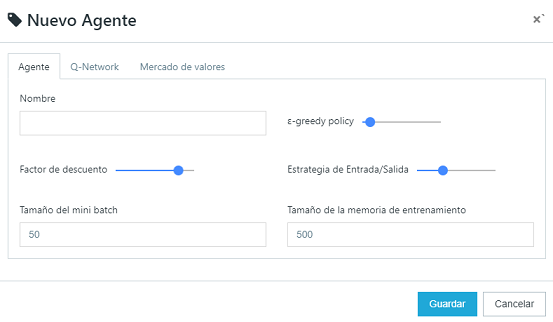
\includegraphics[scale=0.5]{imagenes/screen1.png}
	\end{subfigure}%
	
	 \begin{subfigure}[b]{0.33\textwidth}
		\centering
		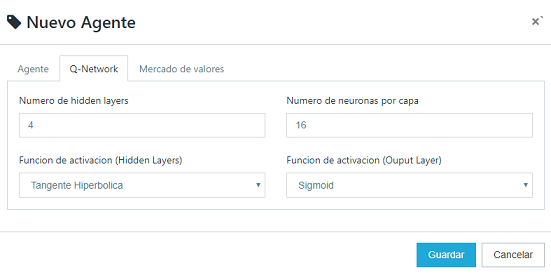
\includegraphics[scale=0.5]{imagenes/screen2.png}
	\end{subfigure}

	 \begin{subfigure}[b]{0.33\textwidth}
		\centering
		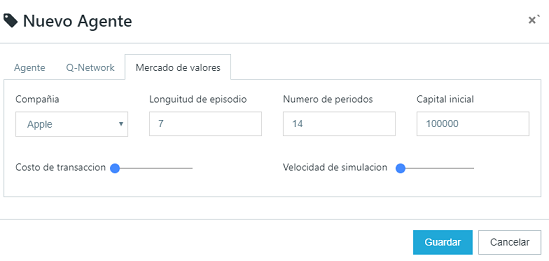
\includegraphics[scale=0.5]{imagenes/screen3.png}
	\end{subfigure}
	
	\caption{Creación de agentes}
	\label{fig:cap4:2}	
\end{figure*}


Cada vez que se cree un agente, se creará también un entorno de simulación con el cual el agente deberá interactuar. El mismo será responsable de la generación de los estados, así como también de los diferentes indicadores bursátiles y del calculo de cada rewards $r_t$. Se podrá inicializar con diferentes opciones, como por ejemplo:

\begin{itemize}
	\item Compañía a tradear
	\item Capital inicial
	\item Costo de transacción
	\item Longitud de episodio (días)
\end{itemize}


Una vez creado el entorno, se podrá acceder a una panel (Figura \ref{fig:cap4:3}) donde se podrá ver la evolución historia que ha tenido la compañía asociada al agente. Desde este panel podrá darse inicio a la simulación, pausarla o eliminar el agente y sus datos asociados. 
Una vez iniciada la simulación, podrá visualizarse en tiempo real, en todos los clientes que estuvieran viendo dicho agente, como va tomando las decisiones de compra o venta, junto con un resumen general del progreso, donde podrá verse
entre otras cosas, el capital actual, la ganancia acumulada, cantidad de acciones que posee el agente, etc.

\begin{figure}[h!]
	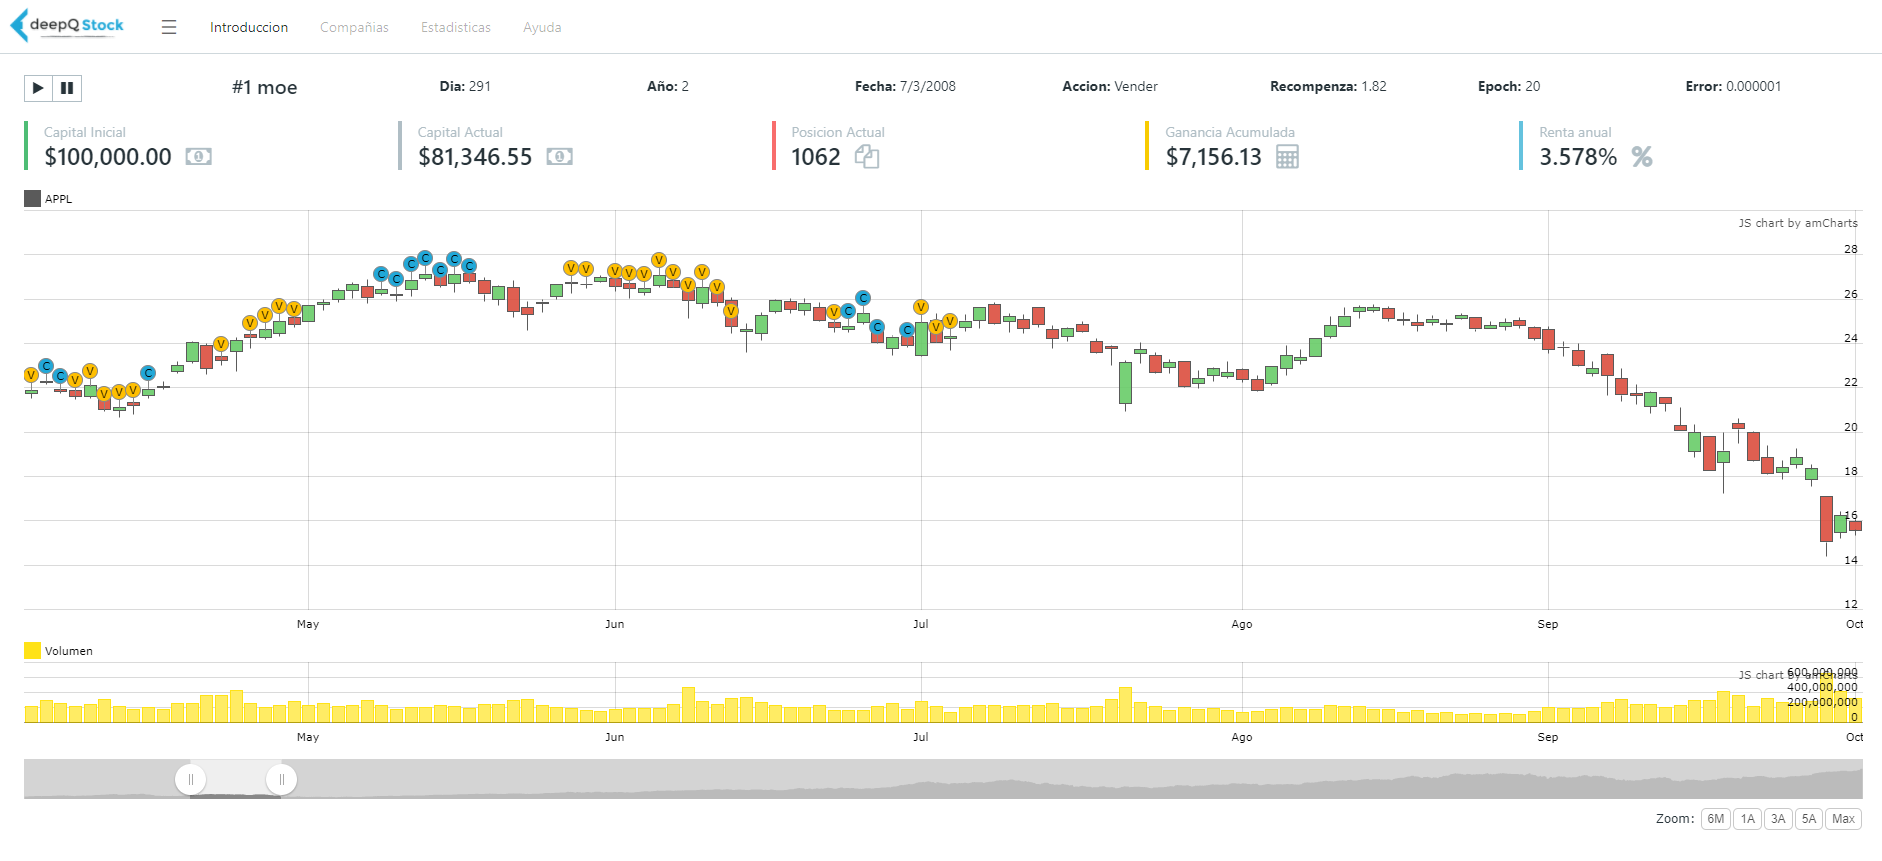
\includegraphics[scale=0.3]{imagenes/screen4.png}
	\caption{Evolución del agente}
		\label{fig:cap4:3}
\end{figure}


Desde la pantalla de creación también podrá setearse parámetros de configuración del agente, como por ejemplo:
\begin{itemize}
	\item Policy $\varepsilon$-greedy, este parámetro representara la frecuencia con la que el agente elegiría en forma aleatoria la próxima acción.
	\item Factor de descuento, este parámetro permitirá configurar el nivel de valoración que se le dará a los rewards mas cercanos en el tiempo.
	\item Tamaño del mini-batch, este representa el tamaño de cada mini batch que el agente utilizara para entrenar a su Q-Network después de la finalizacion de cada episodio.
	\item Tamaño de la memoria de entrenamiento, este parámetro determinara la capacidad de recordar experiencias del agente.
\end{itemize}

\subsection{Aplicación backend}

La aplicación de backend(Figura \ref{fig:cap4:1}) fue implementada en .NET, consta de una servidor de backend, implementado con SignalR 2, SQL Server, Hangfire y Redis. 
Los clientes conectados con la aplicación de angular, se comunicaran con el backend a través de un hub de comunicación implementado con signalR 2, este hub es el que permitirá la comunicación bi-direccional en tiempo real, es decir, desde aplicación cliente hacia el server backend, como desde el server hacia los clientes conectados con la aplicación angular. Este es un requerimiento necesario, dado que los agentes y los simuladores son ejecutados en threads independientes, para lograr esto se necesito integrar el backend con hangfire, un servidor de jobs. 
Cada vez que se inicie la ejecución de un agente, se solicitara a hangfire la creación de un nuevo job o worker, donde se ejecutara el agente y el entorno simulado. El agente comenzara a trader en el entorno configurado para el, e ira notificando a través de una cola de mensajes implementada con redis, todas las decisión y el progreso que esta teniendo al servicio de backend, una vez que el servicio de backend es notificado por redis, este utilizara el hub de comunicación para notificar a el clientes que estén subscritos a escuchar los mensajes de progreso de dicho agente.

\section{Descripción del código}
A continuación describiremos algunas secciones mas relevantes e interesantes del código implementado en el backend.

\subsection{Clase StockExchange}

Esta clase es la que representa nuestro entorno, en nuestro caso, un mercado financiero, ella sera la responsable de calcular los rewards y de ir actualizando los estados $s_t$. También sera responsable de la inicializacion de agente como así también del salvado del estado del agente cada vez q el proceso de ejecución sea pausado. El punto de entrada de esta clase sea el método Simulate() (Figura \ref{fig:cap4:4}).
Como se puede observar en la imagen, este método sera el responsable de la generación de los estados y de la simulación de cada episodio. Cada episodio estará compuesto por una cantidad n de días, en el que en cada día, el agente
deberá tomar una decisión acerca de su situación, es decir, deberá decidir, si compra, vende o espera. Al finalizar cada episodio, el entorno invocara al método OnEpisodeComplete que como se vera mas adelante sera el responsable de entrenamiento de la red neuronal del agente.\\

\begin{figure}[h!]
	\centering
	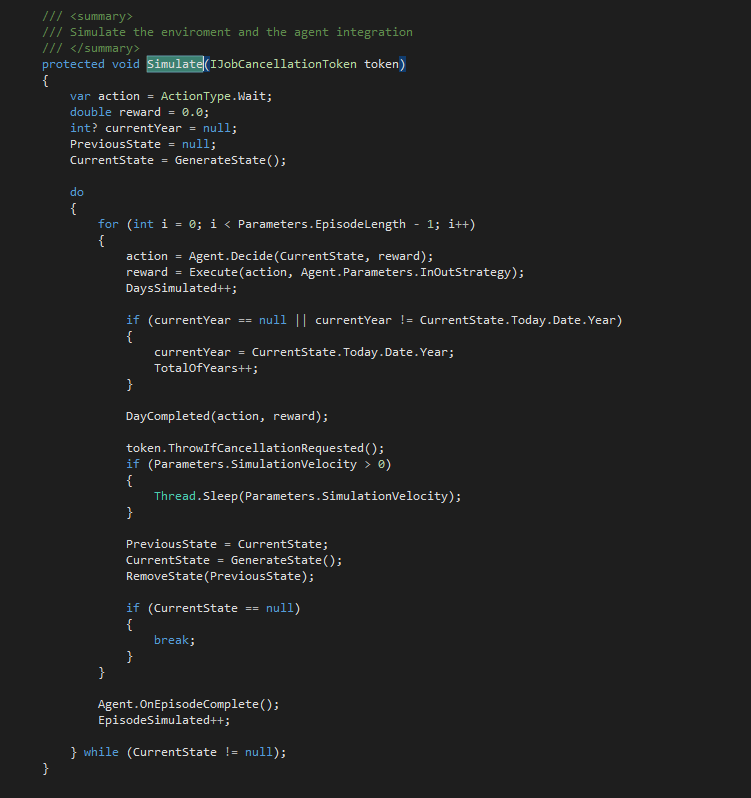
\includegraphics[scale=0.7]{imagenes/screen5.png}
	\caption{Método Simulate}
	\label{fig:cap4:4}
\end{figure}

\clearpage
\subsection{Clase DeepRLAgent}

Esta clase es la que implementa al agente, en ella se implementara la policy de decisión usada por el agente, así como también la Q\_Network y los métodos necesarios para entrenarla.
Como podemos ver, el agente usara este método para decidir(Figura \ref{fig:cap4:5}) en base a una $policy_\pi$
\begin{figure}[h!]
	\centering
	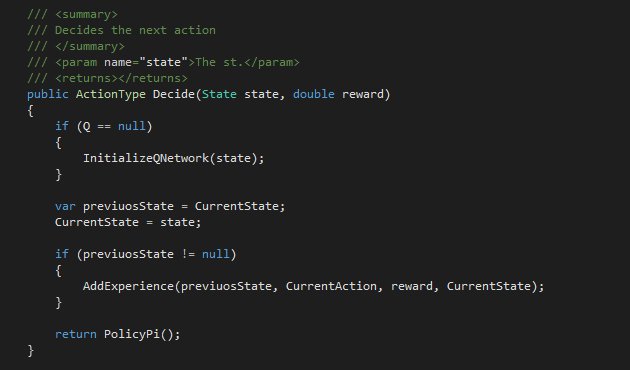
\includegraphics[scale=0.6]{imagenes/screen6.png}
	\caption{Método Decide()}
	\label{fig:cap4:5}
\end{figure}

Se decidió optar por una policy $\varepsilon-greedy$, la cual consiste en elegir siempre la acción que maximiza el reward esperado, según la función estado-acción $Q^*(s_t, a_t)$ con una probabilidad $\varepsilon$ de elegir aleatoriamente, lo cual le permitirá balancear el dilema de exploración vs explotación

\begin{figure}[h!]
	\centering
	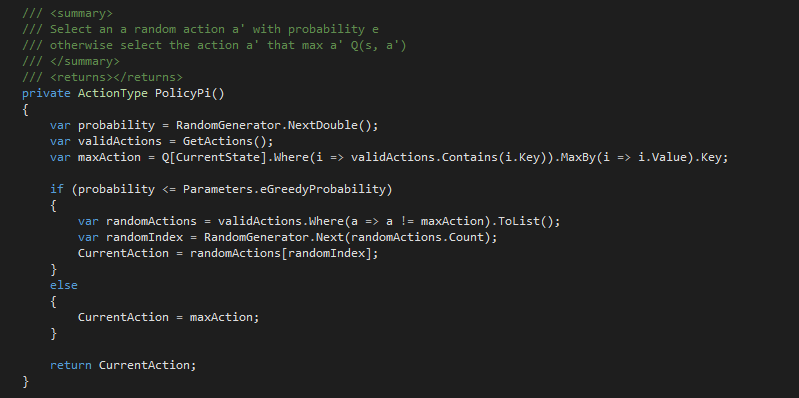
\includegraphics[scale=0.5]{imagenes/screen7.png}
	\caption{Método PolicyPi()}
	\label{fig:cap4:6}
\end{figure}

Por ultimo, una vez finalizado un episodio se ejecutara el método UpdateUknowledge (Figura \ref{fig:cap4:7}) el cual sera el responsable de re-entrenar la red neuronal. Como podemos ver en la imagen, el método generar un mini batch según los parámetros seteados durante la creación del agente, para luego generar los samples de entrenamiento en base a la estimación actual y al valor actualizado usando el algoritmo de Q-learning.
\begin{figure}[h!]
	\centering
	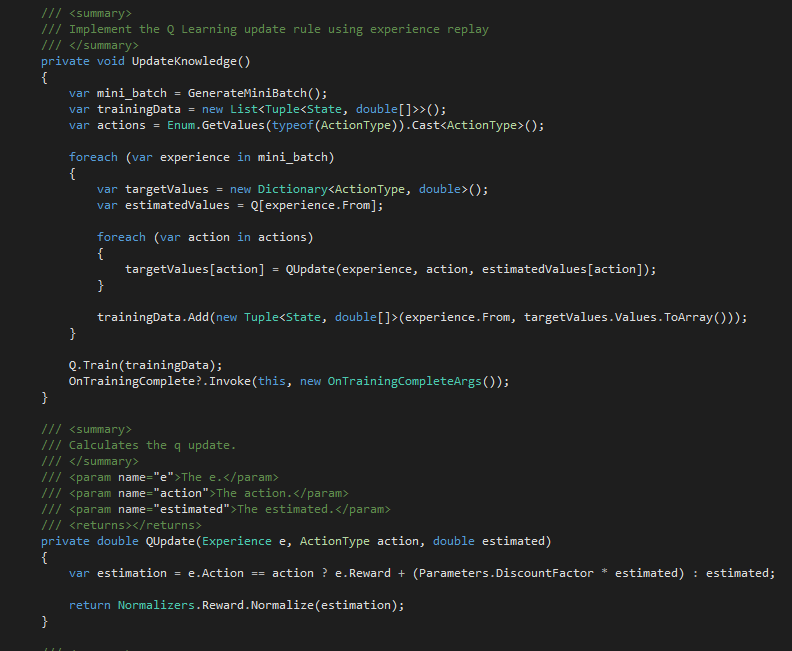
\includegraphics[scale=0.7]{imagenes/screen8.png}
	\caption{Método UpdateUknowledge()}
	\label{fig:cap4:7}
\end{figure}

\begin{figure}[h!]
	\centering
	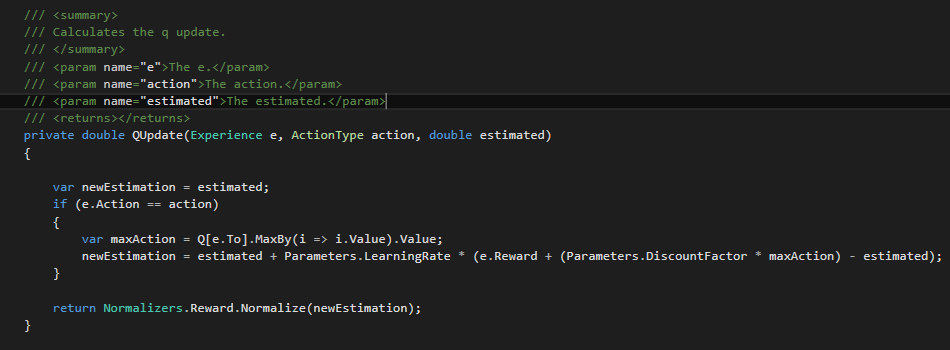
\includegraphics[scale=0.7]{imagenes/screen9.png}
	\caption{Método QUpdate()}
	\label{fig:cap4:8}
\end{figure}